% -------------------- Packages --------------------

\documentclass{assignment}[2019/10/15]
\usepackage[lineno]{packages}[2019/11/14]

% -------------------- Settings --------------------

% Title

\title{Report for Hyperbolic Equations: Solitons}
\author{Chen Xuyang}
\date{\today}
\institute{School of Mathematical Science}
\professor{Chen Suqin}
\course{Numerical Partial Differential Equations}
\subject{Numerical Partial Differential Equations}
\keywords{}

% -------------------- New commands --------------------

\newcommand{\BR}{\symbb{R}}
\newcommand{\BZ}{\symbb{Z}}
\newcommand{\diag}{\mathop{}\!\symup{diag}}
\newcommand{\pr}{\mathop{}\!\symup{Pr}}
\newcommand{\expect}{\mathop{}\!\symup{E}}
\newcommand{\cov}{\mathop{}\!\symup{Cov}}
\newcommand{\var}{\mathop{}\!\symup{Var}}
\newcommand{\mi}{\symup{i}}
\newcommand{\me}{\symup{e}}

\def\multiset#1#2{\ensuremath{\left(\kern-.3em\left(\genfrac{}{}{0pt}{}{#1}{#2}\right)\kern-.3em\right)}}

\newcommand{\lr}[3]{\left#1#3\right#2}
\newcommand{\lmr}[5]{\left#1#4\middle#2#5\right#3}

% -------------------- Document --------------------

\begin{document}
    \maketitle
    \tableofcontents
    \clearpage

    \section{Background}

    \begin{quote}
        ``I believe I shall best introduce this phenomenon by describing the circumstances of my own first acquaintance with it. I was observing the motion of a boat which was rapidly drawn along a narrow channel which it had put in motion; it accumulated round the prow of the vessel in a state of violent agitation, then suddenly leaving it behind, rolled forward with great velocity, assuming the form of a large solitary elevation, a rounded, smooth and well defined heap of water, which continued its course along the channel apparently without change of a form or diminution of speed. I followed it on horse back, and overtook it still rolling on at a rate of some eight or nine miles an hour, preserving its original figure some thirty feet long and a foot to a foot and a half in height. Its height gradually diminished, and after a chase of one or two miles I lost it in the windings of the channel."
    \end{quote}

    In 1895, Korteweg and de Vries formulated the equation
    \begin{equation}\label{eqn: KdV}
        u_t - 6uu_x + u_{xxx} = 0,
    \end{equation}
    which models Russell's observation. The term $uu_x$ describes the sharpening of the wave and $u_{xxx}$ the dispersion (i.e., waves with different wave lengths propagate with different velocities).

    \section{Questions}

    \begin{enumerate}[1)]
        \item Show using direct substitution that the one-soliton solution
        \begin{equation}\label{eqn: one-s}
            u_1(x, t) = -\frac{v}{2\cosh^2\left(\frac{1}{2}\sqrt{v}(x-vt-x_0)\right)}
        \end{equation}
        solves the KdV \ref{eqn: KdV}. Here, $v>0$ and $x_0$ are arbitrary parameters.
        \item We will solve the KdV equation numerically using the method of lines and finite difference approximations for the space derivatives. Rewrite the equation as
        \begin{equation}\label{eqn: KdVm}
            \frac{\partial u}{\partial t} = 6 uu_x - u_{xxx},
        \end{equation}
        and derive a second-order accurate difference approximation of the right-hand side.
        \item For the time integration, we will use a fourth order Runge-Kutta scheme:
        \begin{equation}
            \begin{aligned}
                \alpha^1 &= \Delta tf(u^i)\\
                \alpha^2 &= \Delta tf(u^i+\alpha^1/2)\\
                \alpha^3 &= \Delta tf(u^i+\alpha^2/2)\\
                \alpha^4 &= \Delta tf(u^i+\alpha^3)\\
                u^{i+1} &= u^i + \frac{1}{6}(\alpha^1+2\alpha^2+2\alpha^3+\alpha^4).
            \end{aligned}
        \end{equation}
        The Stability region for this scheme consists of all $z$ such that $\left\vert 1+z+z^2/2+z^3/6+z^4/24\right\vert\leq 1$. In particular, all points on the imaginary axis between $\pm \mi 2\sqrt{2}$ are included.

        Our \ref{eqn: KdV} is non-linear, and to make a stability analysis we first have to linearize it. In this case, it turns out that the stability will be determined by the discretization of the third-derivative term $u_{xxx}$. Therefore, consider the simplified problem
        \begin{equation}
            \frac{\partial u}{\partial t} = - u_{xxx},
        \end{equation}
        and use von Neumann stability analysis to derive an expression for the maximum allowable time-step $\Delta t$ in terms of $\Delta x$.
        \item Write a program that solves the equation using your discretization. Solve it in the region $-8\leq x\leq 8$ with a grid size $\Delta x=0.1$, and use periodic boundary conditions:
        \begin{equation}
            x(-8) = x(8).
        \end{equation}
        Integrate from $t=0$ to $t=2$, using an appropriate time-step that satisfies the condition you derived above. For each of the initial conditions below, plot the solution at $t=2$ and comment on the results.
        \begin{enumerate}[a.]
            \item To begin with, use a single soliton \ref{eqn: one-s} as initial condition, that is, $u(x, 0) = u_1(x, 0)$. Set $v=16$ and $x_0 = 0$.
            \item The one-soliton solution looks almost like a Gaussian. Try $u(x, 0)=-8\me^{-x^2}$.
            \item Try the two-soliton solution $u(x, 0) = -6/\cosh^2(x)$.
            \item Create ``your own" two-soliton solution by superposing two one-soliton solutions with $v=16$ and $v=4$ (both with $x_0=0$).
            \item Same as before, but with $v=16, x_0=4$ and $v=4, x_0=-4$. Describe what happens when the two solitons cross (amplitudes, velocities), and after they have crossed.
        \end{enumerate}
    \end{enumerate}

    \section{Verification for One-Soliton Solution}

    Since it only needs a direct calculatioin of the partial derivatives to verify that one-soliton solution \ref{eqn: one-s} solves the KdV \ref{eqn: KdV} which does not exceed the category of elementry calculus, we shall omit the computions here and check it by the symbolic tool box of MATLAB instead. The following code \ref{mat: q1} will print the sentence
    \begin{quote}
        ``The one-soliton solution solves the KdV equations."
    \end{quote}
    to the screen.

    \matlabinputlisting[caption={Verification for One-Soliton Solution}, label={mat: q1}]{q1.m}

    \section{Construction of a Second-Order Accurate Scheme for the Space Derivatives}

    It can be concluded from the definition that, there are $2p+1 = 2\lr\lfloor\rfloor{(m+1)\middle /2}-1+n$ central coefficients $a_{-p}, a_{-p+1}, \dotsc, a_{p-1}, a_p$ for the $m$-th derivative with accuracy $n$, given by the solution of the linear equation system
    \begin{equation}
        \begin{pmatrix}
            1 & 1 & \cdots & 1 & 1\\
            -p & -p+1 & \cdots & p-1 & p\\
            (-p)^2 & (-p+1)^2 & \cdots & (p-1)^2 & p^2\\
            \cdots & \cdots & \cdots & \cdots & \cdots\\
            \cdots & \cdots & \cdots & \cdots & \cdots\\
            \cdots & \cdots & \cdots & \cdots & \cdots\\
            (-p)^{2p} & (-p+1)^{2p} & \cdots & (p-1)^{2p} & p^{2p}\\
        \end{pmatrix}
        \begin{pmatrix}
            a_{-p}\\
            a_{-p+1}\\
            a_{-p+2}\\
            \cdots\\
            \cdots\\
            \cdots\\
            a_p\\
        \end{pmatrix}
        =
        \begin{pmatrix}
            0\\
            0\\
            0\\
            \cdots\\
            m!\\
            \cdots\\
            0\\
        \end{pmatrix},
    \end{equation}
    where the only non-zero value on the right hand side is in the $m+1$-th row. Thus for a second-order accurate scheme for the third derivative, we have $p=2$ and
    \begin{equation}
        \begin{pmatrix}
            a_{-2}\\
            a_{-1}\\
            a_{0}\\
            a_1\\
            a_2\\
        \end{pmatrix}
        =
        \begin{pmatrix}
            -1/2\\
            1\\
            0\\
            -1\\
            1/2\\
        \end{pmatrix}.
    \end{equation}
    Then we can derive a second-order accurate scheme for the right hand side of modified KdV \ref{eqn: KdVm} as
    \begin{equation}\label{eqn: semi-disc}
        \text{r.h.s.}_k = \frac3{\Delta x}u_k(u_{k+1}-u_{k-1}) - \frac{1}{2(\Delta x)^3}(u_{k+2}-2u_{k+1}+2u_{k-1}-u_{k-2}).
    \end{equation}

    \section{Von Neumann Stability Analysis for Space and Time Discretization}

    We use the scheme \ref{eqn: semi-disc} developed in the previous section to obtain an ordinary equation system of $u_1=u(x_{\text{min}}, t), \dotsc, u_N = u(x_{\text{max}}-\Delta x, t)$, where $N = (x_{\text{max}}-x_{\text{min}})/\Delta x$.

    \section{Numerical Solver and Solutions}

    In the funtion \ref{mat: rhs} \matlabinline{rhs}, we discrete the space derivatives and obtain the ordinary function system $u'=f(u)$. Since a periodic boundary condition is assumed, we don't need to derive a special scheme for the points near the boundary. Instead, we can prolongate the unknown function periodically, i.e. $u_{-2}=u_{N+3}$, to get the value we need in the discretization of space derivatives. To apply this idea elegently, we first prolongate the vector of $u$ by adding $p=2$ elements to the both side of the vector periodically. Then we return the object values by slicing the ``fat" vector, which helps us to deal with the whole vector, including the points near the boundary, at one time with very little additional space complexity.

    \matlabinputlisting[caption={rhs.m}, label={mat: rhs}]{rhs.m}

    In the function \ref{mat: RK44} \matlabinline{RungeKutta44}, we provide a similar interface of the built-in function \matlabinline{ode45}, where we should notice that the functions $u$ and $f$ must have the time parameter before the space parameters, which is in contrary to the form in this problem.

    \matlabinputlisting[caption={RungeKutta44.m}, label={mat: RK44}]{RungeKutta44.m}

    Finally the funtion \ref{mat: solver} \matlabinline{solver} is the main interface of our solver of the KdV equation \ref{eqn: KdV} with periodic boundary condition, as its name shows.

    \matlabinputlisting[caption={solver.m}, label={mat: solver}]{solver.m}

    \begin{figure}[htb]
        \begin{subfigure}[b]{0.3\textwidth}
            \centering
            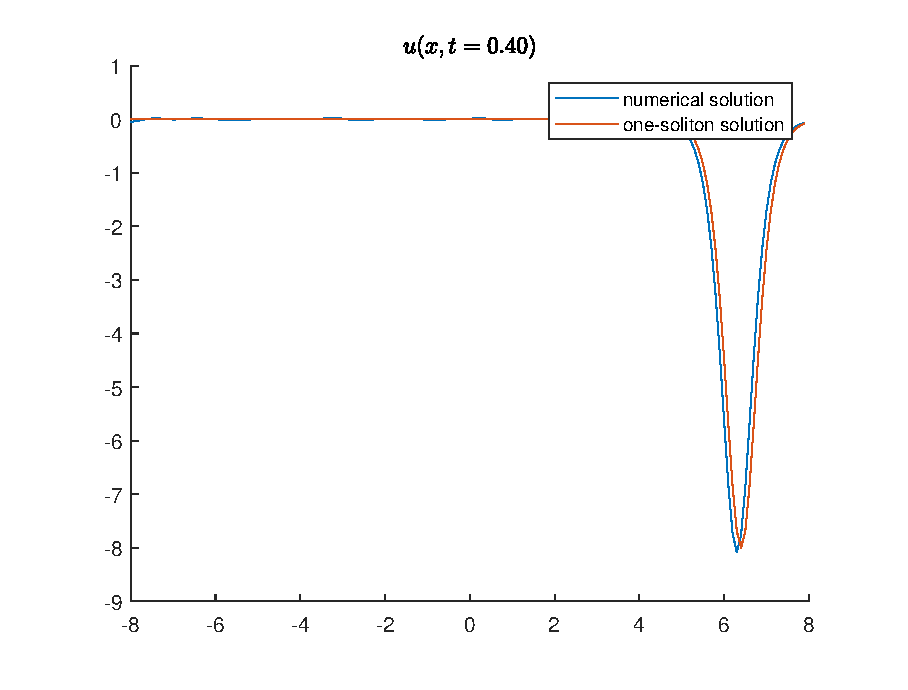
\includegraphics[width=0.3\textwidth]{qa1.eps}
            \caption{$t=0.4$}
        \end{subfigure}
        \hfill
        \begin{subfigure}[b]{0.3\textwidth}
            \centering
            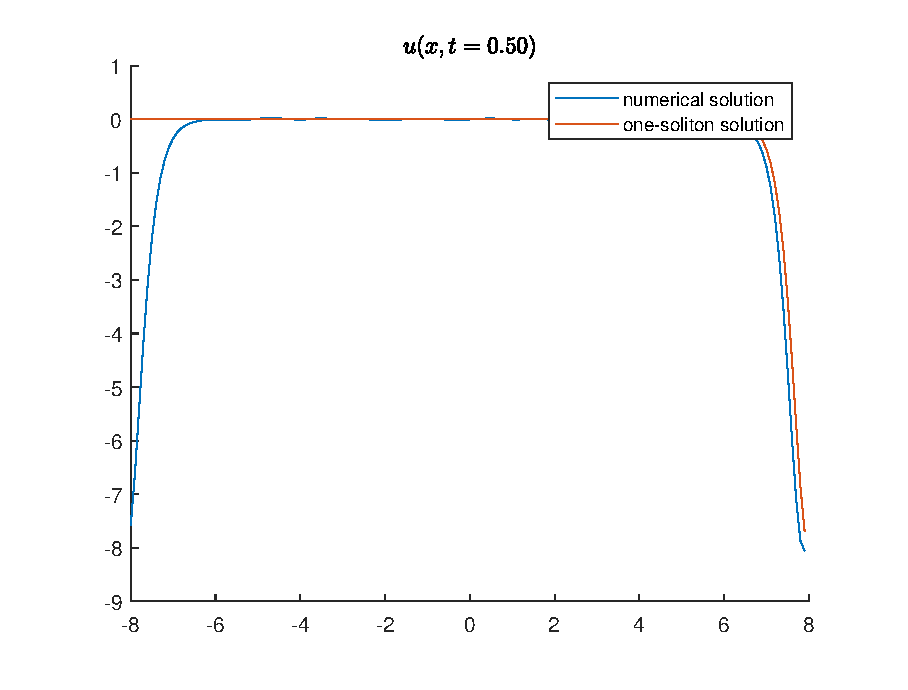
\includegraphics[width=0.3\textwidth]{qa2.eps}
            \caption{$t=0.5$}
        \end{subfigure}
        \hfill
        \begin{subfigure}[b]{0.3\textwidth}
            \centering
            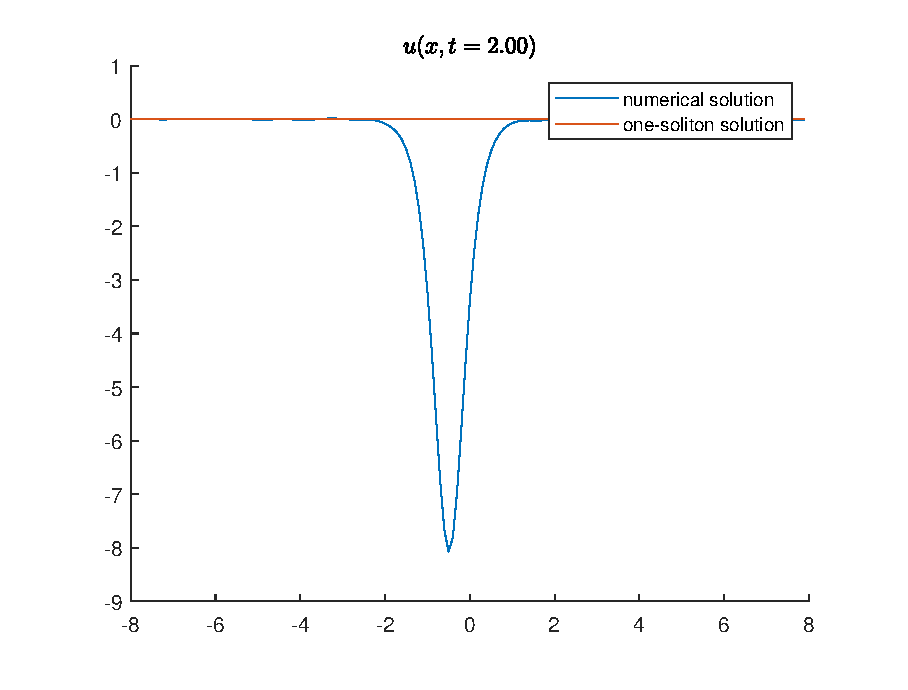
\includegraphics[width=0.3\textwidth]{qa3.eps}
            \caption{$t=2.0$}
        \end{subfigure}
        \caption{Discretization Grid and Contour Lines of the Solutions for $N = 21, l = 3.0, b = 0.5, h = 1.0$.}
        \label{fig: qa}
    \end{figure}
\end{document}
